\documentclass[11pt,a4paper]{report}

\usepackage[margin=1in]{geometry}
\usepackage{titlesec}
\usepackage{tabularx}
\usepackage{longtable}
\usepackage{booktabs}
\usepackage{enumitem}
\usepackage{hyperref}
\usepackage{xcolor}
\usepackage{fancyhdr}
\usepackage{graphicx}
\usepackage{amsmath}
\usepackage{tikz}
\usetikzlibrary{shapes,arrows.meta,positioning,fit}

\definecolor{headcolor}{RGB}{15,70,60}
\hypersetup{
    colorlinks=true,
    linkcolor=headcolor,
    urlcolor=headcolor,
    citecolor=headcolor,
    pdftitle={Software Requirements Specification - TrustBazaar},
    pdfauthor={S. M. Nihal Ahmed}
}

\titleformat{\chapter}[hang]{\normalfont\huge\bfseries\color{headcolor}}{\thechapter}{20pt}{}
\titleformat{\section}{\normalfont\Large\bfseries\color{headcolor}}{\thesection}{10pt}{}
\titleformat{\subsection}{\normalfont\large\bfseries}{\thesubsection}{8pt}{}

\pagestyle{fancy}
\fancyhf{}
\fancyhead[L]{Software Requirements Specification}
\fancyhead[R]{TrustBazaar}
\fancyfoot[C]{\thepage}
\renewcommand{\headrulewidth}{0.4pt}

\newenvironment{reqtable}{\begin{longtable}{p{2.2cm}p{11.5cm}}}{\end{longtable}}
\newenvironment{deftable}{\begin{longtable}{p{3.5cm}p{10.2cm}}}{\end{longtable}}

\title{
    \vspace{-2cm}
    {\Large Daffodil International University}\\[0.3cm]
    {\large Department of Software Engineering}\\[1.5cm]
    \rule{\linewidth}{0.5pt}\\[0.4cm]
    {\huge \textbf{Software Requirements Specification}}\\[0.3cm]
    {\Large TrustBazaar: A Verified Peer-to-Peer Auction \\ and Marketplace Platform for Used Goods}\\[0.4cm]
    \rule{\linewidth}{0.5pt}\\[1cm]
}
\author{
    S. M. Nihal Ahmed \\
    BSc in Software Engineering \\
    Daffodil International University (DIU) \\
    \\
    Prepared for: Capstone Project
}
\date{Version 1.0 \\ \today}

\begin{document}

\maketitle
\thispagestyle{empty}

\vspace{2cm}
\begin{center}
\begin{tabular}{|l|l|}
\hline
\textbf{Document Status} & Draft for Review \\ \hline
\textbf{Version} & 1.0 \\ \hline
\textbf{Prepared By} & S. M. Nihal Ahmed \\ \hline
\textbf{Date} & \today \\ \hline
\textbf{Standard Followed} & IEEE 830-1998 SRS Template \\ \hline
\end{tabular}
\end{center}

\newpage
\thispagestyle{empty}
\tableofcontents
\newpage

\chapter{Introduction}

\section{Purpose}
This Software Requirements Specification (SRS) describes the functional and non-functional requirements for \textbf{TrustBazaar}, a web-based, peer-to-peer marketplace platform on which individuals sell pre-owned items to other individuals through either a fixed-price listing or a time-boxed auction, with identity-verified sellers, escrow-protected payments through local mobile financial services and cards, an integrated logistics/delivery layer, and in-app negotiation via real-time chat. This document is intended to serve as the single point of reference for the system's scope, behavior, data model, and quality attributes throughout design, implementation, testing, and academic evaluation. It follows the structure recommended by IEEE Std 830-1998.

\section{Document Conventions}
Functional requirements are labeled \textbf{FR-\#}, non-functional requirements \textbf{NFR-\#}, both numbered sequentially and grouped by feature area. Priorities follow the MoSCoW convention (\textbf{Must Have}, \textbf{Should Have}, \textbf{Could Have}, \textbf{Won't Have this release}). The words \textbf{shall}/\textbf{must} denote mandatory behavior; \textbf{should} denotes recommended but non-mandatory behavior. Monetary amounts are expressed in Bangladeshi Taka (BDT) unless stated otherwise.

\section{Intended Audience and Reading Suggestions}
\begin{itemize}[nosep]
    \item \textbf{Evaluation panel / course supervisor} -- Chapters 1, 2, 3, and 9 (business model) give the fastest overview of scope and industrial justification.
    \item \textbf{Development team members} -- Chapter 4 (Functional Requirements) and Chapter 6 (Data Model) are the primary implementation references, organized so each feature area can be assigned to a sub-team.
    \item \textbf{Reviewers of quality attributes} -- Chapter 7 (Non-Functional Requirements) details performance, security, and compliance obligations, several of which are specific to handling KYC documents and real money.
\end{itemize}

\section{Project Scope}
TrustBazaar is a single web platform, not a mobile-native app, targeting individual-to-individual resale of used goods within Bangladesh. It is explicitly \textbf{not} a general e-commerce storefront for new/branded retail, and it is explicitly \textbf{not} a management information system: there is no administrative module whose sole purpose is CRUD over inventory, customers, or orders. Instead, the system exists to solve four coupled, non-trivial problems:
\begin{enumerate}[nosep]
    \item Establishing trust between two strangers transacting for real money over an item neither has a pre-existing relationship with (\textbf{KYC verification} and \textbf{escrow-held payment});
    \item Running a fair, tamper-resistant \textbf{time-boxed auction} alongside conventional fixed-price sale, under concurrent multi-user load;
    \item Coordinating \textbf{fulfilment} between two individuals, either via a self-arranged local meetup or a third-party courier with system-computed fare, split automatically between courier and platform; and
    \item Sustaining the platform financially through a small number of clearly modeled \textbf{revenue streams} layered on top of the same settlement transaction.
\end{enumerate}
Real-time chat, ratings, dispute handling, and notification delivery support these four pillars but are not, individually, the system's central technical claim.

\section{Definitions, Acronyms, and Abbreviations}
\begin{deftable}
KYC & Know Your Customer -- identity verification process using a government-issued document. \\
MFS & Mobile Financial Service (e.g., bKash, Nagad) -- Bangladesh's dominant mobile payment rails. \\
Escrow & Funds held by the platform after payment and released to the seller only after buyer confirmation or timeout. \\
Anti-sniping & Automatic auction time extension triggered by a bid placed near the scheduled end time. \\
Ledger & An immutable, itemized record of how a single payment was split among parties (seller, courier, platform). \\
SSE & Server-Sent Events, used for one-directional real-time updates (e.g., live bid counters). \\
NID & National Identity Card (Bangladesh). \\
\end{deftable}

\section{References}
\begin{itemize}[nosep]
    \item IEEE Std 830-1998, IEEE Recommended Practice for Software Requirements Specifications
    \item bKash Merchant / Payment Gateway API Documentation
    \item Nagad Merchant API Documentation
    \item Stripe API Documentation (card payments, webhook signature verification)
    \item Representative Bangladeshi courier fare structures: Pathao Courier, Sundarban Courier Service, RedX, Steadfast Courier (publicly published rate cards)
    \item OWASP Top 10 (2021); OWASP guidance on handling personally identifiable information
    \item Bangladesh Data Protection Act (draft/prevailing regulatory guidance on personal data handling), for KYC document storage practice
\end{itemize}

\chapter{Overall Description}

\section{Product Perspective}
TrustBazaar is a new, self-contained system composed of the following subsystems:
\begin{enumerate}[nosep]
    \item \textbf{Web Client} -- listing browse/search, listing detail with live auction state, chat, checkout, seller dashboard, KYC submission wizard.
    \item \textbf{Core API / Application Backend} -- authentication, listing management, auction engine, order and settlement logic, delivery decision engine, notification dispatch.
    \item \textbf{Real-Time Layer} -- WebSocket/SSE server for live bid updates, countdown synchronization, chat delivery, and outbid/notification push.
    \item \textbf{Payment Layer} -- integrations with bKash, Nagad, and card processing (Stripe or a local acquirer), plus the internal escrow ledger.
    \item \textbf{Delivery Layer} -- distance computation, self-pickup vs. courier decision, courier fare lookup/booking, and delivery-fee revenue split.
    \item \textbf{Data Layer} -- relational database holding users, KYC records, listings, bids, orders, ledger entries, chat, reviews, and disputes.
\end{enumerate}

\section{Product Functions (Summary)}
The system shall allow a user to: register and complete KYC verification; list an item for fixed-price sale or auction; browse, search, and filter listings; place bids on an active auction or purchase a fixed-price item outright; chat in real time with a counterparty about a specific listing; pay via bKash, Nagad, or card into an escrow-protected transaction; choose or be assigned a fulfilment method (self-pickup or courier) with a single blended price; confirm receipt to release escrowed funds, or open a dispute; rate a completed counterparty; and, for sellers, optionally boost a listing or subscribe to a Pro Seller tier.

\section{User Classes and Characteristics}
\begin{itemize}[nosep]
    \item \textbf{Unverified User} -- registered, may browse and chat, but cannot list items or bid/buy until KYC is approved.
    \item \textbf{Verified Individual User} -- completed KYC; may act as buyer and/or seller; default role for the platform.
    \item \textbf{Pro Seller (subscribed)} -- verified user with an active paid subscription granting a lower commission rate, higher concurrent listing limits, and a storefront analytics view.
    \item \textbf{Delivery/Courier Partner (external)} -- not a platform end user in the UI sense, but an integration partner whose API the system calls; may be simulated via a mock service for demonstration purposes.
    \item \textbf{Platform Operator} -- restricted internal role for KYC review, dispute adjudication, and operational monitoring; this is a support function required by the trust model, not a general management console (see Section 2.6 for the explicit boundary).
\end{itemize}

\section{Operating Environment}
\begin{itemize}[nosep]
    \item \textbf{Client:} any evergreen browser (Chrome, Firefox, Safari, Edge) supporting WebSockets and Server-Sent Events.
    \item \textbf{Backend runtime:} Node.js 20+ (NestJS/Express) or Python 3.11+ (FastAPI/Django), containerized with Docker.
    \item \textbf{Database:} PostgreSQL 15+, chosen specifically for strong transactional (ACID) guarantees required by bidding and settlement.
    \item \textbf{Cache/Queue/Real-time backing store:} Redis 7+, used for auction countdown state, bid locks, and pub/sub fan-out to WebSocket connections.
    \item \textbf{Geospatial computation:} PostGIS extension or application-level Haversine distance calculation.
\end{itemize}

\section{Design and Implementation Constraints}
\begin{itemize}[nosep]
    \item All payment integrations (bKash, Nagad, card) shall use official sandbox/test-mode credentials; no real financial transactions shall be processed in the academic deliverable.
    \item Courier integration shall use a real courier's published sandbox API where available; where no public sandbox exists, a mock courier service reproducing realistic fare and status-update behavior shall be substituted, and this substitution shall be explicitly documented, not presented as a live integration.
    \item KYC document images shall be stored encrypted at rest and shall never be exposed via a directly guessable or public URL.
    \item The Platform Operator role described in Section 2.4 shall be strictly limited to KYC review and dispute adjudication queues; it shall not provide generic create/edit/delete access to listings, users, or orders, in order to preserve the system's identity as a marketplace rather than a management system.
\end{itemize}

\section{User Documentation}
Deliverables include this SRS, a System Design Document (data model, sequence diagrams, API contracts), a README with Docker Compose setup instructions, and in-app contextual help for the KYC submission flow and the auction bidding rules (including anti-sniping behavior, which must be explained to first-time bidders).

\section{Assumptions and Dependencies}
\begin{itemize}[nosep]
    \item It is assumed that bKash and Nagad sandbox developer access can be obtained for the academic project; if unavailable, Stripe test mode alone shall be used and this limitation documented.
    \item It is assumed that server-side clocks (used for auction countdown authority) are synchronized via NTP; auction fairness depends on this.
    \item Courier fare figures are assumed to be reasonable approximations of real published rate cards rather than certified real-time quotes, unless a live sandbox is available.
\end{itemize}

\chapter{System Features}
Each feature below lists its purpose, priority, and associated functional requirement range detailed in Chapter 4.

\section{Feature 1: Account Registration and KYC Verification}
\textbf{Description:} Users register with email/phone and password, then submit a government ID and a selfie for identity verification before being permitted to list items or transact. \textbf{Priority:} Must Have. \textbf{Requirements:} FR-1 to FR-9.

\section{Feature 2: Listing Creation (Fixed-Price and Auction)}
\textbf{Description:} A verified seller creates a listing choosing either a fixed price with available stock count, or an auction with a starting price, reserve price (optional), and duration. \textbf{Priority:} Must Have. \textbf{Requirements:} FR-10 to FR-18.

\section{Feature 3: Search and Discovery}
\textbf{Description:} Buyers browse and filter listings by category, price, condition, distance, and listing type (auction/fixed). \textbf{Priority:} Must Have. \textbf{Requirements:} FR-19 to FR-22.

\section{Feature 4: Auction Engine}
\textbf{Description:} Server-authoritative bidding with anti-sniping extension, proxy (automatic) bidding, reserve price enforcement, live bid feed, and automatic winner determination. \textbf{Priority:} Must Have. \textbf{Requirements:} FR-23 to FR-34.

\section{Feature 5: Fixed-Price Purchase}
\textbf{Description:} Concurrency-safe stock decrement so that simultaneous buyers cannot both purchase the last unit of a listing. \textbf{Priority:} Must Have. \textbf{Requirements:} FR-35 to FR-38.

\section{Feature 6: Payment and Escrow Settlement}
\textbf{Description:} Collects payment via bKash, Nagad, or card; holds funds in escrow; releases to seller on buyer confirmation or automatic timeout; supports refunds and disputes. \textbf{Priority:} Must Have. \textbf{Requirements:} FR-39 to FR-49.

\section{Feature 7: Delivery and Fulfilment}
\textbf{Description:} Computes buyer-seller distance; recommends self-pickup with a safe meetup point under a distance threshold, or books a courier and quotes a blended price above it; splits the delivery fee between courier and platform. \textbf{Priority:} Should Have. \textbf{Requirements:} FR-50 to FR-58.

\section{Feature 8: Real-Time Chat}
\textbf{Description:} Per-listing buyer-seller messaging, including image sharing, tied to the transaction thread. \textbf{Priority:} Must Have. \textbf{Requirements:} FR-59 to FR-64.

\section{Feature 9: Ratings, Reviews, and Trust Signals}
\textbf{Description:} Post-transaction rating, unlockable only after a completed paid transaction; KYC-verified badge; Pro Seller badge. \textbf{Priority:} Should Have. \textbf{Requirements:} FR-65 to FR-68.

\section{Feature 10: Dispute Resolution}
\textbf{Description:} Buyer-initiated dispute flow that freezes escrow release pending operator adjudication. \textbf{Priority:} Should Have. \textbf{Requirements:} FR-69 to FR-73.

\section{Feature 11: Notifications}
\textbf{Description:} Real-time and asynchronous notifications for outbid events, auction-ending-soon, payment confirmation, delivery status, and new chat messages. \textbf{Priority:} Should Have. \textbf{Requirements:} FR-74 to FR-77.

\section{Feature 12: Monetization Features}
\textbf{Description:} Transaction commission, delivery-fee margin, featured/boosted listings, and Pro Seller subscription. \textbf{Priority:} Must Have (commission, delivery margin); Could Have (featured listings, subscription). \textbf{Requirements:} FR-78 to FR-86.

\section{Feature 13: Trust and Safety Controls}
\textbf{Description:} Listing reporting/flagging, bid-rate limiting, duplicate-listing fraud heuristics, and audit logging of all monetary and bidding events. \textbf{Priority:} Should Have. \textbf{Requirements:} FR-87 to FR-91.

\chapter{Functional Requirements}

\section{Account Registration and KYC Verification}
\begin{reqtable}
\textbf{FR-1} & The system shall allow a new user to register with an email or phone number and a password. \\
\textbf{FR-2} & The system shall hash and salt passwords using a strong algorithm (bcrypt or argon2); plaintext passwords shall never be stored or logged. \\
\textbf{FR-3} & The system shall issue a short-lived JWT access token and a rotating refresh token upon login. \\
\textbf{FR-4} & The system shall require a registered user to submit a government-issued ID (NID or passport) image and a live selfie before being granted Verified status. \\
\textbf{FR-5} & The system shall store submitted KYC documents encrypted at rest, accessible only to the reviewing operator role and the owning user. \\
\textbf{FR-6} & The system shall track KYC status per user as one of: \texttt{unsubmitted}, \texttt{pending\_review}, \texttt{verified}, \texttt{rejected}, with rejection requiring a reason code. \\
\textbf{FR-7} & The system shall prevent an \texttt{unsubmitted} or \texttt{rejected} user from creating a listing, placing a bid, or completing a purchase, enforced server-side on every relevant request. \\
\textbf{FR-8} & The system shall display a Verified badge on the profile and listings of any user with \texttt{verified} KYC status. \\
\textbf{FR-9} & The system shall allow a rejected user to resubmit KYC documents. \\
\end{reqtable}

\section{Listing Creation}
\begin{reqtable}
\textbf{FR-10} & The system shall allow a Verified user to create a listing with title, description, category, condition (new/like-new/used/for-parts), and one or more photos. \\
\textbf{FR-11} & The system shall require at least two photos per listing, including one clearly showing any visible defects, before publication. \\
\textbf{FR-12} & The system shall allow a seller to choose listing type: \texttt{fixed\_price} or \texttt{auction}, at creation time; the type shall not be changed after the first bid or purchase. \\
\textbf{FR-13} & For a fixed-price listing, the system shall require a price and an available stock quantity of at least 1. \\
\textbf{FR-14} & For an auction listing, the system shall require a starting price, an auction duration (default options of 1 or 2 hours, configurable up to 72 hours), and shall accept an optional hidden reserve price. \\
\textbf{FR-15} & The system shall record the seller's pickup location (approximate, for distance calculation) at listing creation or from the seller's saved profile location. \\
\textbf{FR-16} & The system shall allow a seller to edit a listing's description or photos before any bid or purchase has occurred, but not its price, type, or duration once active. \\
\textbf{FR-17} & The system shall allow a seller to cancel a fixed-price listing with no completed sales at any time; an auction listing with at least one bid shall not be cancelable except by operator intervention. \\
\textbf{FR-18} & The system shall enforce a maximum number of concurrently active listings per seller, higher for Pro Seller accounts than standard Verified accounts. \\
\end{reqtable}

\section{Search and Discovery}
\begin{reqtable}
\textbf{FR-19} & The system shall allow full-text search over listing titles and descriptions. \\
\textbf{FR-20} & The system shall allow filtering results by category, price range, condition, listing type, and maximum distance from the buyer's location. \\
\textbf{FR-21} & The system shall support sorting results by newest, price (ascending/descending), and auction ending soonest. \\
\textbf{FR-22} & The system shall exclude listings whose seller's KYC status is not \texttt{verified} from public search results. \\
\end{reqtable}

\section{Auction Engine}
\begin{reqtable}
\textbf{FR-23} & The system shall maintain the authoritative auction end time on the server; the client shall treat any locally displayed countdown as informational only. \\
\textbf{FR-24} & The system shall accept a bid only if it exceeds the current highest bid by at least a configured minimum increment. \\
\textbf{FR-25} & The system shall process concurrent bids using a transaction-safe mechanism (row-level locking or equivalent) such that two simultaneous bids can never both be recorded as the current highest bid. \\
\textbf{FR-26} & The system shall reject a bid placed after the auction's authoritative end time, even if the client submitted it before observing the end locally. \\
\textbf{FR-27} & The system shall extend the auction end time by a configurable interval (default 2 minutes) whenever a valid bid is placed within that interval of the current end time (anti-sniping). \\
\textbf{FR-28} & The system shall allow a bidder to set a maximum proxy bid amount; the system shall automatically place the minimum necessary incremental bid on the bidder's behalf whenever outbid, up to that maximum. \\
\textbf{FR-29} & The system shall not reveal any bidder's proxy maximum to other bidders or the seller. \\
\textbf{FR-30} & The system shall not declare a winning bid below the seller's reserve price, if one was set; the listing shall instead close as unsold. \\
\textbf{FR-31} & The system shall broadcast live bid updates (new highest bid, time remaining) to all connected clients viewing the auction in real time. \\
\textbf{FR-32} & The system shall notify the outbid bidder in real time when a higher bid is placed. \\
\textbf{FR-33} & Upon auction close, the system shall determine the winning bidder and create a pending order requiring payment within a configured window (default 24 hours). \\
\textbf{FR-34} & If the winning bidder does not complete payment within the window, the system shall offer the item to the next-highest bidder (second-chance offer) before relisting or closing the auction as unsold. \\
\end{reqtable}

\section{Fixed-Price Purchase}
\begin{reqtable}
\textbf{FR-35} & The system shall allow a Verified buyer to purchase a fixed-price listing at the listed price, subject to available stock. \\
\textbf{FR-36} & The system shall decrement stock and create an order within a single atomic transaction, such that concurrent purchase requests cannot both succeed when only one unit remains. \\
\textbf{FR-37} & The system shall mark a fixed-price listing as sold out and remove it from active search results once stock reaches zero. \\
\textbf{FR-38} & The system shall queue purchase requests received during a burst (e.g., a popular relisted item) and process them in order rather than dropping or silently failing excess requests. \\
\end{reqtable}

\section{Payment and Escrow Settlement}
\begin{reqtable}
\textbf{FR-39} & The system shall support payment via bKash, Nagad, and card (Stripe or equivalent) at checkout, in sandbox/test mode for the academic deliverable. \\
\textbf{FR-40} & The system shall confirm payment completion via a server-to-server webhook or callback from the payment provider, not solely via client-side redirect state. \\
\textbf{FR-41} & The system shall process each payment webhook idempotently, such that duplicate delivery of the same payment confirmation event does not create duplicate orders or double-credit any party. \\
\textbf{FR-42} & Upon confirmed payment, the system shall place the full amount (item price plus any delivery fee) into an escrow-held state, not immediately payable to the seller. \\
\textbf{FR-43} & The system shall release escrowed seller funds automatically upon explicit buyer confirmation of receipt, or automatically after a configured timeout (default 5 days) if the buyer takes no action and no dispute is open. \\
\textbf{FR-44} & The system shall record every escrow state transition (\texttt{held}, \texttt{released}, \texttt{refunded}, \texttt{frozen\_disputed}) with a timestamp and triggering actor. \\
\textbf{FR-45} & The system shall support a full or partial refund to the buyer when a dispute is resolved in the buyer's favor. \\
\textbf{FR-46} & The system shall generate a single itemized settlement ledger entry per completed order showing: item price, platform commission, delivery fee, courier payout, and platform delivery margin. \\
\textbf{FR-47} & The system shall reconcile payment gateway state against internal order/escrow state via a periodic background job, to catch missed or delayed webhook deliveries. \\
\textbf{FR-48} & The system shall retry a failed payment-provider API call with exponential backoff up to a configured maximum before surfacing a failure to the user. \\
\textbf{FR-49} & The system shall never store raw card numbers or MFS account credentials; payment provider tokens/references shall be used exclusively. \\
\end{reqtable}

\section{Delivery and Fulfilment}
\begin{reqtable}
\textbf{FR-50} & The system shall compute the distance between buyer and seller locations at checkout using stored approximate coordinates. \\
\textbf{FR-51} & If the computed distance is at or below a configurable threshold (default 2 km), the system shall recommend self-pickup and shall not add a delivery fee. \\
\textbf{FR-52} & For a self-pickup transaction, the system shall suggest at least one safe public meetup point near the midpoint of buyer and seller locations, drawn from a curated list (e.g., police stations, shopping mall entrances). \\
\textbf{FR-53} & The system shall share only approximate location (not exact home address) between buyer and seller prior to an agreed meetup. \\
\textbf{FR-54} & If the computed distance exceeds the self-pickup threshold, the system shall compute a courier delivery fare based on a distance/weight fare model approximating published Bangladeshi courier rate cards. \\
\textbf{FR-55} & The system shall present the buyer a single blended checkout price (item price plus delivery fare) without requiring the buyer to select a specific courier. \\
\textbf{FR-56} & Upon payment confirmation for a courier-fulfilled order, the system shall create a booking request to the integrated (or mocked) courier service, including pickup and drop-off details. \\
\textbf{FR-57} & The system shall track and display delivery status (\texttt{booked}, \texttt{picked\_up}, \texttt{in\_transit}, \texttt{delivered}) to both buyer and seller. \\
\textbf{FR-58} & Upon delivery confirmation, the system shall split the collected delivery fee between the courier payout and the platform's delivery margin according to a configured percentage, recorded in the settlement ledger (FR-46). \\
\end{reqtable}

\section{Real-Time Chat}
\begin{reqtable}
\textbf{FR-59} & The system shall provide a real-time chat thread scoped to a specific listing between the prospective buyer and seller. \\
\textbf{FR-60} & The system shall deliver messages to an online recipient via WebSocket in real time, and shall queue messages for delivery when the recipient reconnects if currently offline. \\
\textbf{FR-61} & The system shall support sharing images within a chat thread. \\
\textbf{FR-62} & The system shall persist full chat history per thread, retrievable by either participant on return. \\
\textbf{FR-63} & The system shall display a delivered/read indicator per message. \\
\textbf{FR-64} & The system shall allow a user to report a chat thread's content as abusive or fraudulent, feeding the trust-and-safety queue (FR-87). \\
\end{reqtable}

\section{Ratings, Reviews, and Trust Signals}
\begin{reqtable}
\textbf{FR-65} & The system shall allow a buyer and seller to rate each other (1--5 stars, optional text) only after an order's escrow has been released or refunded. \\
\textbf{FR-66} & The system shall prevent a rating from being submitted for an order with no completed payment. \\
\textbf{FR-67} & The system shall display a seller's average rating and completed-transaction count on their profile and listings. \\
\textbf{FR-68} & The system shall display distinct badges for KYC-verified status and active Pro Seller subscription. \\
\end{reqtable}

\section{Dispute Resolution}
\begin{reqtable}
\textbf{FR-69} & The system shall allow a buyer to open a dispute against an order within a configured window after delivery/meetup (default 3 days), providing a reason and optional evidence photos. \\
\textbf{FR-70} & Opening a dispute shall immediately transition the order's escrow to \texttt{frozen\_disputed}, preventing automatic timeout release. \\
\textbf{FR-71} & The system shall notify the seller and the Platform Operator queue when a dispute is opened. \\
\textbf{FR-72} & The system shall allow an operator to resolve a dispute with one of: release to seller, refund to buyer (full or partial), requiring a recorded reason. \\
\textbf{FR-73} & The system shall log every dispute state change with timestamp and responsible actor for audit purposes. \\
\end{reqtable}

\section{Notifications}
\begin{reqtable}
\textbf{FR-74} & The system shall send a real-time notification to a bidder when they have been outbid. \\
\textbf{FR-75} & The system shall send a notification when an auction the user is watching or bidding on is within a configured time of ending (default 5 minutes). \\
\textbf{FR-76} & The system shall send a notification on payment confirmation, delivery status change, and new chat message. \\
\textbf{FR-77} & The system shall allow a user to view a unified notification history within the app. \\
\end{reqtable}

\section{Monetization Features}
\begin{reqtable}
\textbf{FR-78} & The system shall deduct a platform commission, expressed as a configurable percentage of item price, from the seller's payout on every completed sale. \\
\textbf{FR-79} & The system shall apply a lower commission percentage to Pro Seller accounts than to standard Verified accounts. \\
\textbf{FR-80} & The system shall retain a configurable percentage of every courier delivery fee as platform delivery margin, per FR-58. \\
\textbf{FR-81} & The system shall allow a seller to pay a flat fee to feature a listing in top-of-search placement or a homepage carousel for a fixed duration. \\
\textbf{FR-82} & The system shall visually distinguish featured listings from organic results without misleading users as to their nature (labeled ``Featured''). \\
\textbf{FR-83} & The system shall offer a recurring Pro Seller subscription granting a lower commission rate, a higher concurrent-listing limit, and a basic sales analytics view. \\
\textbf{FR-84} & The system shall process Pro Seller subscription billing and renewal through the same payment providers used for purchases, with webhook-based confirmation. \\
\textbf{FR-85} & The system shall automatically revert a Pro Seller account to standard status upon subscription cancellation or repeated renewal payment failure. \\
\textbf{FR-86} & The system shall record every commission, delivery-margin, featured-listing, and subscription charge in an auditable revenue log separate from the buyer/seller settlement ledger. \\
\end{reqtable}

\section{Trust and Safety Controls}
\begin{reqtable}
\textbf{FR-87} & The system shall allow any user to report a listing as fraudulent, counterfeit, or misrepresented, adding it to an operator review queue. \\
\textbf{FR-88} & The system shall rate-limit bid submissions per user per auction to mitigate bid-spam or automated bidding abuse outside the proxy-bid mechanism (FR-28). \\
\textbf{FR-89} & The system shall flag for operator review a seller who repeatedly relists an item shortly after a cancelled or disputed sale. \\
\textbf{FR-90} & The system shall maintain an immutable audit log of all bid placements, payment state transitions, and escrow transitions. \\
\textbf{FR-91} & The system shall restrict the Platform Operator role to the KYC review queue, dispute queue, and trust-and-safety report queue; no generic listing/user/order edit capability shall be exposed through this role. \\
\end{reqtable}

\chapter{External Interface Requirements}

\section{User Interfaces}
The web client shall provide, at minimum: a registration/login view; a KYC submission wizard (document upload, selfie capture, status tracker); a listing browse/search view with filters; a listing detail view showing either a fixed-price ``Buy Now'' action or a live auction panel (current highest bid, countdown, bid/proxy-bid input, live bid log); a checkout flow presenting the blended item-plus-delivery price and payment method selection; an order status view (payment, escrow, delivery tracking, confirm-receipt action); a per-listing chat panel; a seller dashboard (active listings, sales, Pro Seller analytics if subscribed); and an operator-only queue view for KYC and disputes, access-restricted per FR-91.

\section{Hardware Interfaces}
No specialized hardware interfacing is required. KYC selfie capture uses the client device's standard camera via the browser's Media Capture API.

\section{Software Interfaces}
\begin{reqtable}
\textbf{bKash API} & Merchant payment initiation, execution, and webhook-based payment confirmation (sandbox). \\
\textbf{Nagad API} & Merchant payment initiation and confirmation (sandbox). \\
\textbf{Card Processor API} & Stripe (test mode) or equivalent, for card payments and subscription billing, with webhook signature verification. \\
\textbf{Courier API (or mock)} & Fare quotation and booking creation; sandbox where available (e.g., Pathao/Steadfast), otherwise a documented internal mock service. \\
\textbf{Geolocation/Distance Service} & Browser Geolocation API for capturing approximate coordinates; server-side Haversine or PostGIS calculation for distance. \\
\textbf{PostgreSQL} & Primary relational data store for all transactional data. \\
\textbf{Redis} & Auction countdown state, bid-lock coordination, WebSocket pub/sub fan-out, rate-limit counters. \\
\end{reqtable}

\section{Communications Interfaces}
All client-server traffic shall use HTTPS. Live auction updates, outbid notifications, and chat delivery shall use WebSocket connections; auction countdown broadcast may alternatively use Server-Sent Events. Payment and courier webhook callbacks shall be received over authenticated HTTPS endpoints and verified using each provider's signature-verification mechanism before being trusted.

\chapter{Data Model Overview}
This chapter summarizes the core entities and their relationships; a full normalized schema is provided in the accompanying System Design Document.

\section{Core Entities}
\begin{reqtable}
\textbf{User} & id, email/phone, password\_hash, kyc\_status, role (standard/pro/operator), location (lat/long). \\
\textbf{KYCDocument} & id, user\_id, document\_type, encrypted\_file\_ref, review\_status, reviewed\_by, reviewed\_at. \\
\textbf{Listing} & id, seller\_id, type (fixed/auction), title, description, category, condition, photos, price or (starting\_price, reserve\_price, end\_time), stock, status. \\
\textbf{Bid} & id, listing\_id, bidder\_id, amount, is\_proxy, proxy\_max, placed\_at. \\
\textbf{Order} & id, listing\_id, buyer\_id, seller\_id, item\_price, delivery\_fee, total, fulfilment\_type, status. \\
\textbf{EscrowTransaction} & id, order\_id, state (held/released/refunded/frozen\_disputed), state\_history. \\
\textbf{SettlementLedger} & id, order\_id, item\_price, platform\_commission, delivery\_fee, courier\_payout, platform\_delivery\_margin, seller\_payout. \\
\textbf{DeliveryRequest} & id, order\_id, fulfilment\_type, distance\_km, courier\_reference, status, meetup\_point (if self-pickup). \\
\textbf{ChatThread / Message} & thread scoped to listing + participants; messages with sender, content, attachment, delivered/read state. \\
\textbf{Review} & id, order\_id, rater\_id, ratee\_id, stars, comment. \\
\textbf{Dispute} & id, order\_id, opened\_by, reason, evidence, status, resolution, resolved\_by. \\
\textbf{Subscription} & id, user\_id, tier, status, renewal\_date, payment\_reference. \\
\textbf{FeaturedListing} & id, listing\_id, start\_at, end\_at, fee\_paid. \\
\end{reqtable}

\section{Key Relationships}
A \emph{User} may own many \emph{Listings}; a \emph{Listing} of type auction has many \emph{Bids} but exactly one winning \emph{Order}; every \emph{Order} has exactly one \emph{EscrowTransaction} and exactly one \emph{SettlementLedger} entry; an \emph{Order} has at most one \emph{DeliveryRequest} and at most one \emph{Dispute}; \emph{Reviews} reference a completed \emph{Order} and are directional (buyer-to-seller and seller-to-buyer are separate rows).

\chapter{Non-Functional Requirements}

\section{Performance Requirements}
\begin{reqtable}
\textbf{NFR-1} & A bid placement request shall be acknowledged (accepted or rejected) within 500 ms under normal load. \\
\textbf{NFR-2} & Live auction state (highest bid, time remaining) shall propagate to all connected viewers of that auction within 1 second of a state change. \\
\textbf{NFR-3} & Search results for a filtered query shall return within 2 seconds for a catalog of up to 100,000 listings, assuming appropriate indexing. \\
\end{reqtable}

\section{Security Requirements}
\begin{reqtable}
\textbf{NFR-4} & KYC document files shall be encrypted at rest and served only via short-lived signed URLs to authorized viewers (the owning user and the reviewing operator). \\
\textbf{NFR-5} & The system shall enforce per-user data isolation such that one user cannot retrieve another user's KYC documents, chat threads, or order details by manipulating identifiers (IDOR protection). \\
\textbf{NFR-6} & All payment and courier webhook endpoints shall verify provider-supplied signatures before processing the payload. \\
\textbf{NFR-7} & The system shall rate-limit authentication, bid-placement, and checkout endpoints to mitigate brute-force and abuse. \\
\textbf{NFR-8} & Secrets (API keys, database credentials, webhook signing secrets) shall be stored in environment variables or a secrets manager, never committed to source control. \\
\end{reqtable}

\section{Reliability and Availability}
\begin{reqtable}
\textbf{NFR-9} & Failed calls to a payment or courier provider shall be retried with exponential backoff up to a configured maximum before the user is shown an error. \\
\textbf{NFR-10} & A periodic reconciliation job shall compare internal escrow/order state against payment-provider state to catch missed webhook events (supports FR-47). \\
\textbf{NFR-11} & The auction countdown authority shall survive a single application server restart without resetting or extending any auction's true end time (state persisted in Redis/DB, not in-process memory). \\
\end{reqtable}

\section{Usability Requirements}
\begin{reqtable}
\textbf{NFR-12} & A first-time bidder shall be able to view the anti-sniping and proxy-bidding rules from the auction detail page without leaving it. \\
\textbf{NFR-13} & The KYC submission wizard shall clearly communicate document requirements and current review status at every step. \\
\end{reqtable}

\section{Maintainability and Portability}
\begin{reqtable}
\textbf{NFR-14} & The backend, database, cache, and real-time service shall run as separate containers orchestrated via Docker Compose. \\
\textbf{NFR-15} & Automated unit tests shall cover, at minimum: concurrent bid processing, concurrent fixed-price stock decrement, payment-webhook idempotency, and the delivery-fee split calculation. \\
\textbf{NFR-16} & A continuous integration pipeline shall run the automated test suite on every push to the main branch. \\
\end{reqtable}

\section{Legal and Compliance Considerations}
\begin{reqtable}
\textbf{NFR-17} & KYC document collection, storage, and retention shall follow applicable Bangladeshi data protection guidance; documents shall be retained no longer than necessary and deletable on account closure. \\
\textbf{NFR-18} & The system shall present clear terms disclosing the platform commission rate and delivery-margin percentage to sellers before listing creation. \\
\end{reqtable}

\section{Scalability Considerations}
\begin{reqtable}
\textbf{NFR-19} & The real-time layer shall use a pub/sub mechanism (Redis pub/sub or equivalent) so that additional application server instances can be added without each needing a direct in-memory reference to every connected client. \\
\textbf{NFR-20} & Database indexes shall be defined on frequently queried columns (\texttt{listing\_id}, \texttt{seller\_id}, \texttt{buyer\_id}, geospatial index on location) to avoid full-table scans as data volume grows. \\
\end{reqtable}

\chapter{System Architecture Overview}

\section{High-Level Component Architecture}
Figure~\ref{fig:architecture} shows the major subsystems and their interactions.

\begin{figure}[h]
\centering
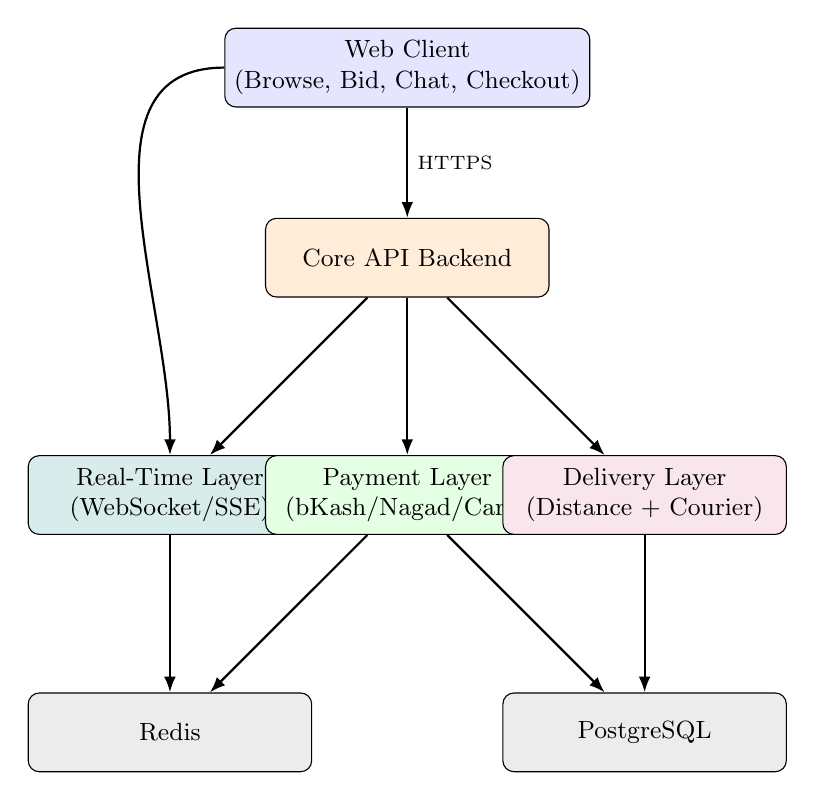
\begin{tikzpicture}[
    box/.style={draw, rounded corners, minimum width=3.6cm, minimum height=1cm, align=center, font=\small},
    arrow/.style={-{Latex[length=2mm]}, thick}
]
\node[box, fill=blue!10] (client) {Web Client\\(Browse, Bid, Chat, Checkout)};
\node[box, fill=orange!15, below=1.4cm of client] (api) {Core API Backend};
\node[box, fill=teal!15, below left=2.0cm and -0.6cm of api] (rt) {Real-Time Layer\\(WebSocket/SSE)};
\node[box, fill=green!10, below=2.0cm of api] (pay) {Payment Layer\\(bKash/Nagad/Card)};
\node[box, fill=purple!10, below right=2.0cm and -0.6cm of api] (delivery) {Delivery Layer\\(Distance + Courier)};
\node[box, fill=gray!15, below=2.0cm of rt] (redis) {Redis};
\node[box, fill=gray!15, below=2.0cm of delivery] (db) {PostgreSQL};

\draw[arrow] (client) to[out=180,in=90] (rt);
\draw[arrow] (client) -- node[right, font=\scriptsize]{HTTPS} (api);
\draw[arrow] (api) -- (rt);
\draw[arrow] (api) -- (pay);
\draw[arrow] (api) -- (delivery);
\draw[arrow] (rt) -- (redis);
\draw[arrow] (pay) -- (db);
\draw[arrow] (delivery) -- (db);
\draw[arrow] (pay) -- (redis);
\end{tikzpicture}
\caption{High-level component architecture of TrustBazaar}
\label{fig:architecture}
\end{figure}

\section{Auction Bid Sequence}
Figure~\ref{fig:bidflow} shows the server-authoritative bid handling sequence, including anti-sniping.

\begin{figure}[h]
\centering
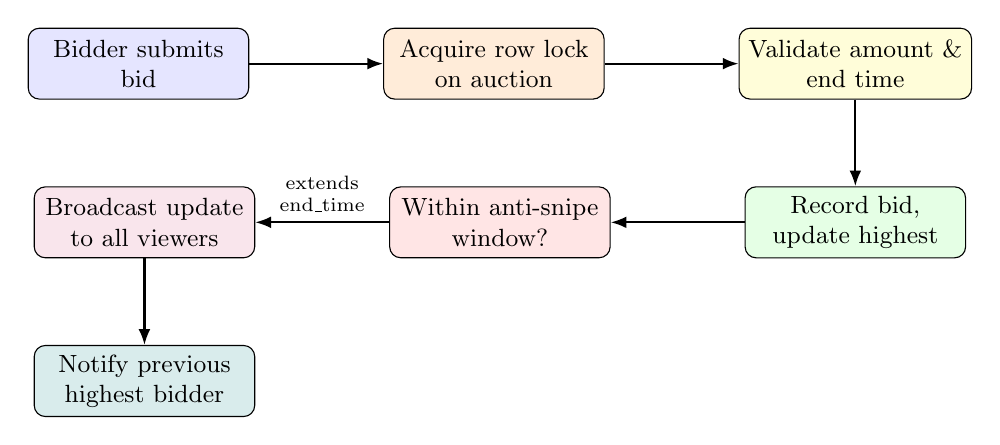
\begin{tikzpicture}[
    node distance=1.1cm and 1.7cm,
    box/.style={draw, rounded corners, minimum width=2.8cm, minimum height=0.9cm, align=center, font=\small},
    arrow/.style={-{Latex[length=2mm]}, thick}
]
\node[box, fill=blue!10] (bid) {Bidder submits\\bid};
\node[box, fill=orange!15, right=of bid] (lock) {Acquire row lock\\on auction};
\node[box, fill=yellow!15, right=of lock] (check) {Validate amount \&\\end time};
\node[box, fill=green!10, below=of check] (accept) {Record bid,\\update highest};
\node[box, fill=red!10, left=of accept] (extend) {Within anti-snipe\\window?};
\node[box, fill=purple!10, left=of extend] (broadcast) {Broadcast update\\to all viewers};
\node[box, fill=teal!15, below=of broadcast] (notify) {Notify previous\\highest bidder};

\draw[arrow] (bid) -- (lock);
\draw[arrow] (lock) -- (check);
\draw[arrow] (check) -- (accept);
\draw[arrow] (accept) -- (extend);
\draw[arrow] (extend) -- node[above, font=\scriptsize, align=center]{extends\\end\_time} (broadcast);
\draw[arrow] (broadcast) -- (notify);
\end{tikzpicture}
\caption{Server-authoritative bid processing with anti-sniping}
\label{fig:bidflow}
\end{figure}

\section{Settlement and Delivery Split Flow}
Figure~\ref{fig:settlement} shows how a single confirmed payment is decomposed into the settlement ledger.

\begin{figure}[h]
\centering
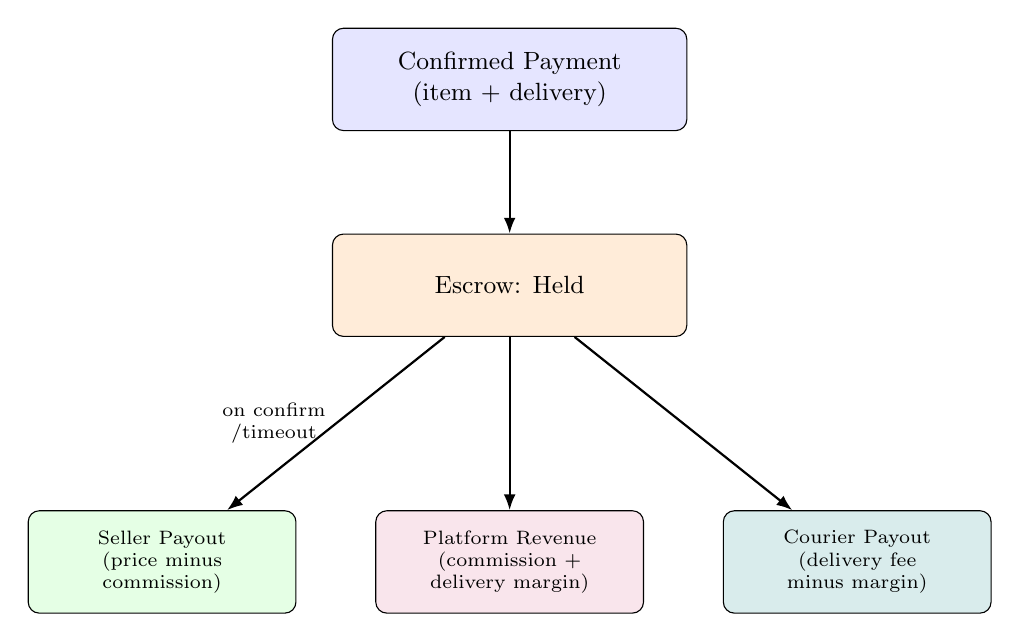
\begin{tikzpicture}[
    node distance=1.2cm and 0.7cm,
    box/.style={draw, rounded corners, minimum width=3.4cm, minimum height=1.3cm, align=center, font=\scriptsize},
    arrow/.style={-{Latex[length=2mm]}, thick}
]
\node[box, fill=blue!10, minimum width=4.5cm, font=\small] (payment) {Confirmed Payment\\(item + delivery)};
\node[box, fill=orange!15, below=1.3cm of payment, minimum width=4.5cm, font=\small] (escrow) {Escrow: Held};
\node[box, fill=purple!10, below=2.2cm of escrow] (platform) {Platform Revenue\\(commission +\\delivery margin)};
\node[box, fill=green!10, left=1.0cm of platform] (seller) {Seller Payout\\(price minus\\commission)};
\node[box, fill=teal!15, right=1.0cm of platform] (courier) {Courier Payout\\(delivery fee\\minus margin)};

\draw[arrow] (payment) -- (escrow);
\draw[arrow] (escrow) -- node[left, font=\scriptsize, align=center]{on confirm\\/timeout} (seller);
\draw[arrow] (escrow) -- (platform);
\draw[arrow] (escrow) -- (courier);
\end{tikzpicture}
\caption{Settlement ledger split on order completion}
\label{fig:settlement}
\end{figure}

\chapter{Business Model and Revenue Design}

\section{Revenue Streams}
\begin{longtable}{p{3.3cm}p{3.6cm}p{5.9cm}}
\toprule
\textbf{Stream} & \textbf{Trigger} & \textbf{Model} \\
\midrule
Transaction commission & Completed sale (fixed-price or auction) & Percentage of item price, deducted at seller payout (lower rate for Pro Sellers) \\
Delivery margin & Courier-fulfilled delivery & Percentage of buyer-paid delivery fee retained before courier payout \\
Featured listings & Seller opts to boost & Flat fee per fixed duration (e.g., 24/48 hours) \\
Pro Seller subscription & Recurring opt-in & Monthly flat fee; grants lower commission, higher listing limits, analytics \\
Buyer protection add-on (optional) & High-value item checkout & Flat fee or small percentage for extended dispute coverage \\
\bottomrule
\end{longtable}

\section{Implementation Priority}
The transaction commission and delivery margin streams are treated as \textbf{Must Have} since they reuse the settlement ledger already required by Feature 6 and 7 at no additional architectural cost. Featured listings and the Pro Seller subscription are treated as \textbf{Could Have}, fully designed in this document but subject to time-boxing during implementation.

\chapter{Appendix}

\section{Appendix A: Auction Rule Summary}
\begin{reqtable}
\textbf{Minimum increment} & Configurable, e.g., 2\% of current bid or a flat minimum, whichever is greater. \\
\textbf{Anti-sniping window} & Default 2 minutes before scheduled end; a qualifying bid extends the end time by 2 minutes. \\
\textbf{Proxy bidding} & Bidder sets a private maximum; system bids the minimum increment above the next-highest bid automatically, up to that maximum. \\
\textbf{Reserve price} & Hidden minimum; auction closes unsold if not met. \\
\textbf{Payment window} & 24 hours after auction close for winner to pay, else second-chance offer to next-highest bidder. \\
\end{reqtable}

\section{Appendix B: Delivery Decision Thresholds}
\begin{reqtable}
\textbf{$\leq$ 2 km} & Self-pickup recommended; safe public meetup point suggested; no delivery fee. \\
\textbf{$>$ 2 km} & Courier booking with system-quoted blended fare; fee split between courier payout and platform margin. \\
\end{reqtable}

\section{Appendix C: Glossary}
\begin{deftable}
Escrow & Platform-held funds between payment and confirmed delivery/receipt. \\
Anti-sniping & Automatic auction extension to prevent last-second unfair bidding. \\
Proxy bid & An automatically incrementing bid up to a hidden maximum set by the bidder. \\
Settlement ledger & Auditable record of how one payment was divided among seller, courier, and platform. \\
KYC & Identity verification using a government-issued document and a live selfie. \\
\end{deftable}

\end{document}